\section{Die Normalform komplexer Zahlen}
\subsection{Die imaginäre Einheit \texorpdfstring{$i$}{i}}

%Der Ausgangspunkt, um die reellen Zahlen zu den komplexen Zahlen zu erweitern, ist die Gleichung $x^2 = -1$, die in $\R$ aufgestellt, aber nicht gelöst werden kann (das Quadrat einer reellen Zahl ungleich null ist stets positiv). 

\begin{definition}{Die imaginäre Einheit $i$}{}
Die \textit{imaginäre Einheit} $i$ ist eine Zahl, welche die Gleichung $x^2=-1$ erfüllt. Es gilt also: 
$$i^2=-1$$
\end{definition}

Bisher wissen wir nur, dass $i$ keine reelle Zahl ist, da das Quadrat einer reellen Zahl nicht negativ sein kann. Was genau wir uns unter $i$ vorstellen sollten, ist noch nicht ganz klar. Dennoch können wir bereits mit $i$ rechnen, da gemäss dem dritten Punkt des Permanenzprinzips die Rechenregeln aus $\mathbb{R}$ auch für die komplexen Zahlen weiterhin gültig bleiben:



\begin{satz}{Rechnen mit $i$}{}
    \begin{itemize}
        \item Mit der imaginären Einheit $i$ wird gerechnet wie mit einer Variablen.
        \item Alle zweiten und höheren Potenzen von $i$ werden mit Hilfe der Relation $i^2 = -1$ ersetzt.
    \end{itemize}
    \end{satz}

    \begin{bsp}{Rechnen mit $i$}{}
        $i \cdot (3 - (5-3i)) = $

        \vspace*{1cm}

        $i^3 = $
        %\vspace*{1cm}
    \end{bsp}

    \begin{bsp}
    {Neu lösbare Gleichung}{}
    Die Gleichung $x^2 = -4$ ist in der Grundmenge der reellen Zahlen nicht lösbar. Lässt man imaginäre Ergebnisse zu, hat die Gleichung jedoch zwei Lösungen:

    \vspace*{2cm}


    \end{bsp}

    \emph{Bemerkung:}
Man sollte $i$ nicht einfach als $\sqrt{-1}$ schreiben, weil dies in den reellen Zahlen nicht definiert ist. Wenn man mit diesem Wurzelsymbol so rechnet, wie man das aus dem Reellen gewöhnt ist, dann stösst man schnell auf Widersprüche.\footnote{Früheren Mathematikern war die Zahl $i$ übrigens etwas unheimlich. GOTTFRIED WILHELM LEIBNIZ (1646-1716) beispielsweise nannte sie „ein Amphibium zwischen Sein und Nichtsein“, für LEONHARD EULER (1707-1783) war sie eine „unmögliche Zahl“, und noch KARL FRIEDRICH GAUSS (1777-1855) bezeichnete sie im neunzehnten Jahrhundert als „Schatten von Schatten“. Da $i$ also eine „unmögliche Zahl“ war, das heisst keine reelle Zahl, nannte man sie „imaginär" (von lateinisch imaginarius $=$ eingebildet). Die Bezeichnung geht auf RENÉ DESCARTES (1596-1650) zurück.}
$$1=\sqrt{1}=\sqrt{(-1)\cdot(-1)}=\sqrt{-1}\cdot \sqrt{-1}=i\cdot i=-1$$


\begin{ueb}{Erstes Rechnen mit der imaginären Einheit}{uebungzui}
    \begin{enumerate}
        \item Berechnen Sie die Potenzen von $i$:

\begin{enumerate}
	\item $i^2=$
	\item $i^3=$
	\item $i^4=$
	\item $i^5=$
	\item $i^6=$
	\item $i^7=$
	\item $i^{123}=$
\end{enumerate}


\textbf{Beobachtung:} %Die Potenzen von $i$ wiederholen sich in einem Zyklus von vier.

\item Berechnen Sie die folgenden Ausdrücke.

\begin{enumerate}
    \item $i^7 + i^9 + i^{12} + i^4$
    \item $i(-i) + (-i)^2 + i^4 - i^3 - (-i)^4$
    \item $\frac{i^{12} \cdot i^{10} \cdot i^{20}}{i^{44}}$
    \item $(2i - i^3)^2 + (i + 3i^2)^2$
\end{enumerate}
\item Lösen Sie die folgenden quadratischen Gleichungen.

\begin{enumerate}
    \item $x^2 = -9$
    \item $x^2 = -15$
    \item $x^2 + 2x + 2 = 0$
\end{enumerate}
\end{enumerate}
\end{ueb}


\clearpage
\emph{Lösungen}
\begin{enumerate}
\item Berechnen Sie die Potenzen von $i$:
    \begin{enumerate}
        \item $i^2= -1$
        \item $i^3= -i$
        \item $i^4= 1$
        \item $i^5= i$
        \item $i^6= -1$
        \item $i^7= -i$
        \item $i^{123}= -i$
    \end{enumerate}
    
    \item Berechnen Sie die folgenden Ausdrücke:
    \begin{enumerate}
        \item $i^7 + i^9 + i^{12} + i^4 = -i +i +1 +1 = 2$
        \item $i(-i) + (-i)^2 + i^4 - i^3 - (-i)^4 = 1 + (-1) + 1 + i -1 = i$
        \item $\frac{i^{12} \cdot i^{10} \cdot i^{20}}{i^{44}} = -1$
        \item $(2i - i^3)^2 + (i + 3i^2)^2 = -1-6i$
    \end{enumerate}
    
    \item Lösen Sie die folgenden quadratischen Gleichungen:
    \begin{enumerate}
        \item $x^2 = -9 \Rightarrow x = \pm 3i$
        \item $x^2 = -15 \Rightarrow x = \pm \sqrt{15}i$
        \item $x^2 + 2x + 2 = 0 \Rightarrow x = -1 \pm i$
    \end{enumerate}
\end{enumerate}
















\clearpage
\subsection{Die Normalform}
Alle Ergebnisse der \Cref{uebng:uebungzui} sind Zahlen der Form $a+b\cdot i$ mit $a,\ b\in \R$. Letztere bilden die Menge der komplexen Zahlen:

\begin{definition}{Normalform einer komplexen Zahl}{}
\emph{Komplexe Zahlen} sind Zahlen der Form $z=a+b\cdot i$, wobei $a,\ b\in \R$ sind. 

Die Menge der komplexen Zahlen ist: 
$$\C=\left\{a+bi \, | \, a,\ b\in \R\right\}$$

Die reelle Zahlen $a$ bzw. $b$ nennt man \emph{Realteil} bzw.  \emph{Imaginärteil} der komplexen Zahl $z=a+bi$:

$$\RE(a+bi)=a \hspace{4cm} \IM(a+bi)=b$$

Eine Zahl, deren Realteil $0$ ist, nennt man \emph{rein imaginär}.


\end{definition}

\begin{bsp}
{}{}
Bei der Zahl $z = 3-9i$ handelt es sich um eine komplexe Zahl mit
$$\RE(z)=3 \hspace{4cm} \IM(z)=-9$$

\end{bsp}

\begin{itemize}
	\item Das Wort „komplex“ steht hier für „zusammengesetzt“ (Latein complexus = verflochten), da alle komplexe Zahlen aus einem reellen Anteil und einem imaginären Anteil zusammengesetzt sind.
	\item Jede reelle Zahl ist auch eine komplexe Zahl (mit Imaginärteil $0$). Beispiel $-42=-42+0i$.\\	Die Menge $\R$ ist also eine Teilmenge der Menge $\C$:
	$$\textcolor{ForestGreen}{\N}\subset\textcolor{Brown}{\Z}\subset\textcolor{BrickRed}{\Q}\subset\textcolor{RoyalBlue}{\R}\subset\textcolor{DarkOrchid}{\C}$$
\end{itemize}


\begin{center}
    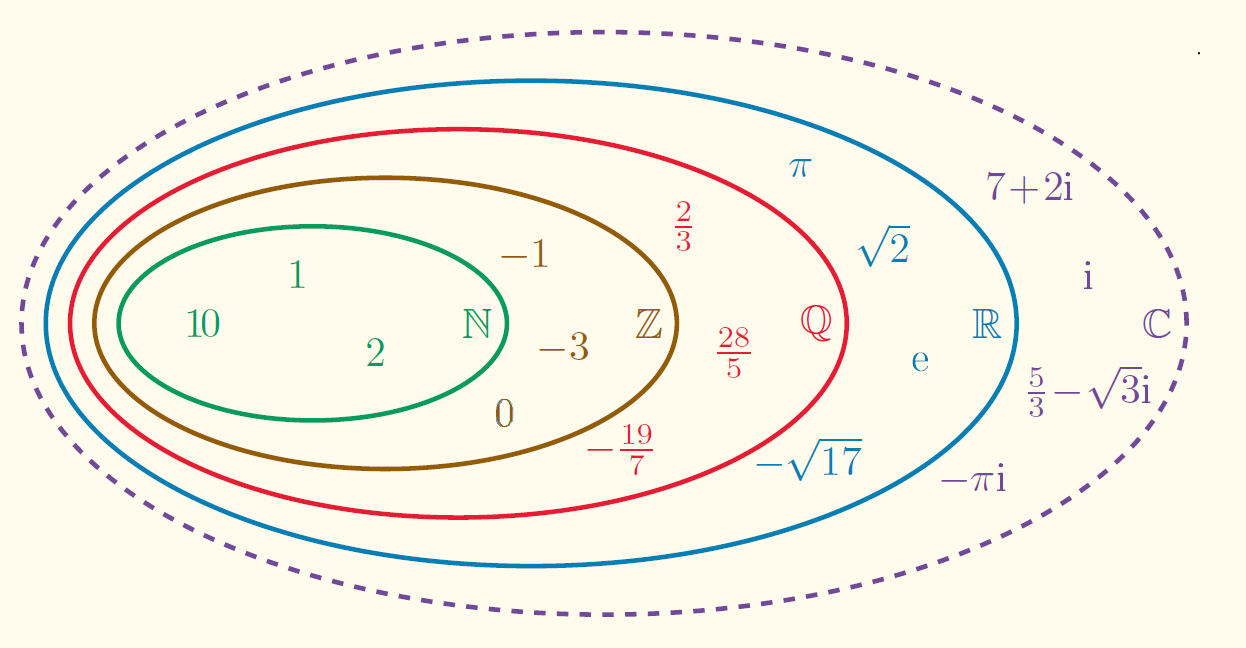
\includegraphics[width = 0.75 \textwidth]{media/zahlenmengen.png}
\end{center}

Bei den beiden Lösungen $x_1 = -1 + i$ und $x_2 = -1 - i$ der Gleichung $x^2 + 2x + 2 = 0$ (Siehe \Cref{uebng:uebungzui}) fällt auf, dass sie sich nur durch im Vorzeichen des Imaginärteils unterscheiden. Solche Zahlen werden konjugiert komplexe Zahlen genannt.

\begin{definition}
    {Die konjugiert komplexe Zahl}{}
    Die zu $z = a + bi$ konjugiert komplexe Zahl $\bar{z}$ ist definiert als 
    $$\bar{z} = a - bi$$

\end{definition}

\begin{ueb}
    {Übungen zur Normalform}{uebZuNormalform}
    \begin{enumerate}
        \item Geben Sie Realteil und Imaginärteil der folgenden komplexen Zahlen an
    
        \begin{enumerate}
            \item $z=-1+4 i$ \hfill $\RE(z)=\phantom{aaaa}$ \hspace{2.5cm} $\IM(z)=\phantom{aaaa}$\hspace{3cm}\phantom{a}
            \item $z=2-5 i$ \hfill $\RE(z)=\phantom{aaaa}$ \hspace{2.5cm} $\IM(z)=\phantom{aaaa}$\hspace{3cm}\phantom{a}
        
            \item $z=-\frac{1}{6}$\hfill $\RE(z)=\phantom{aaaa}$ \hspace{2.5cm} $\IM(z)=\phantom{aaaa}$\hspace{3cm}\phantom{a}
            \item $z=i-\pi$\hfill $\RE(z)=\phantom{aaaa}$ \hspace{2.5cm} $\IM(z)=\phantom{aaaa}$\hspace{3cm}\phantom{a}
        
        \end{enumerate}
        \item Sind die folgenden Aussagen richtig oder falsch? Begründen Sie Ihre Antworten.
        \begin{itemize}
            \item Für alle komplexen Zahlen $z$ gilt: $z=\RE(z)+\IM(z)$.
            \item Für alle komplexe Zahlen $z$ mit $\RE(\IM(z))=0$ gilt: $z \in \R$.
        \end{itemize}
        \item Setzen Sie  $z = a + bi$ und zeigen Sie damit, dass die folgenden Aussagen gelten:
        \begin{enumerate}
            \item $\bar{\bar{z}}= z$
            \item $z + \bar{z} = 2\operatorname{Re}(z) = 2a \in \mathbb{R}$
            \item $z - \bar{z} = 2i\operatorname{Im}(z) = 2bi$ (rein imaginär)
             \item  $z \cdot \bar{z} = a^2 + b^2 \in \mathbb{R}$
            \item $z = \bar{z} \iff z \in \mathbb{R}$
            % \item $\overline{z + w}  = \bar{z} + \bar{w}$
        \end{enumerate}

    \end{enumerate}
\end{ueb}


\clearpage
\emph{Lösungen}
\begin{enumerate}
    \item Geben Sie Realteil und Imaginärteil der folgenden komplexen Zahlen an:
    \begin{enumerate}
        \item $\RE(z)=-1$, $\IM(z)=4$
        \item $\RE(z)=2$, $\IM(z)=-5$
        \item $\RE(z)=-\frac{1}{6}$, $\IM(z)=0$
        \item $\RE(z)=-\pi$, $\IM(z)=1$
    \end{enumerate}
    
    \item Sind die folgenden Aussagen richtig oder falsch?
    \begin{itemize}
        \item Falsch
        \item Wahr
    \end{itemize}
    
    \item 
    Bei der Beweisführung ist darauf zu achten, dass man die Behauptung durch kleinschrittigen Umformungen zeigt. 
    \begin{enumerate}
        \item $\bar{\bar z} = \overline{\overline{a+bi}} = \overline{a-bi} = \overline{a+(-b)i} = a-(-b)i = a+bi = z$ 
        \item $z + \bar{z} = (a+bi) + \overline{a+bi} = a+bi + a-bi = 2a$
        \item $z - \bar{z} = (a+bi) - \overline{a+bi} = a+bi -(a-bi) = 2bi$
        \item $z \cdot \bar{z} = (a+bi)\cdot(a-bi) = a^2 - (bi)^2 = a^2 -b^2i^2 = a^2-b^2\cdot (-1) = a^2+b^2$
        \item $z = \bar{z} \iff a+bi = a-bi \iff b = -b \iff b=0 \iff \IM(z)=0 \iff  z \in \R$
    \end{enumerate}
\end{enumerate}















\clearpage
\subsection{Grundoperationen mit komplexen Zahlen}
Bei allen Grundoperationen werden die Terme so zusammengefasst, dass das Endergebnis in der Normalform $a+bi$ steht. 

\begin{bsp}{Addition und Subtraktion}{}
     Gegeben sind die komplexe Zahlen $z=-3-5i$ und $w=2+7i$.
$$z+w=-3-5i+2+7i=\phantom{fdjskaljfkdsljfkslkl}$$
	\vfill
    $$z-w=-3-5i-(2+7i)=\phantom{fdjskaljfkdsljfksl}$$
    \vfill

\end{bsp}

\begin{satz}{Addition und Subtraktion komplexer Zahlen}{}
Für $z=a + bi$ und $w=c + di$ mit $a,\ b,\ c,\ d\in \R$ gilt:\\

$\displaystyle{(a + bi) + (c + di) =}$ \\

$\displaystyle{(a + bi) - (c + di) =}$


\end{satz}

\begin{bsp}{Multiplikation und Division}{}
    Gegeben sind die komplexe Zahlen $z=-3-5i$ und $w=5+12i$. 

    \bigskip

$z\cdot w=(-3-5i)\cdot (5+12i)=\phantom{fdjskaljfkdsljfkslkl}$

   \vspace*{2cm}

   $\frac{z}{w}=\frac{-3-5i}{5+12i}=\phantom{fdjskaljfkdsljfksl}$
   \vspace*{3cm}

\end{bsp}

\begin{satz}
    {Multiplikation und Division komplexer Zahlen}{}
    Für $z=a + bi$ und $w=c + di$ mit $a,\ b,\ c,\ d\in \R$ gilt:\\

    $\displaystyle{(a + bi) \cdot (c + di) =}$\\
    
    $\displaystyle{\frac{a+bi}{c+di} =}$
\end{satz}

\begin{ueb}
    {Zu den Grundoperationen}{Grundoperationen}
    \begin{enumerate}
        \item Berechnen Sie für $v=6-i$, $w=4$ und $z=5i$ die folgenden Ausdrücke:
        \begin{enumerate}
            \item $v+w=$
            \vfill
            \item $3v+\overline{w}-z=$
            \vfill
            \item $\RE(z+5w)=$
            \vfill
            \item $\IM(z-w)=$
            \item $v\cdot z=$
            \vfill
            \item $v\cdot w\cdot i=$
            \vfill
            \item $\frac{w}{v}=$
            \vfill
            \item $\frac{v}{z}=$
            \vfill
            \item $v^2=$
            \end{enumerate}
        \item Geben Sie das Resultat in Normalform an:
        \begin{enumerate}
            \item $\displaystyle{\frac{1}{1+2i}=}$\vfill
            \item $\displaystyle{\frac{\overline{5+3i}}{1-i}}=$\vfill
            \item $(2i-3)^3=$\vfill
            \item $i+i^{-1}=$\vfill
        \end{enumerate}
        \item Zeigen Sie, dass die komplexe Konjugation mit den vier Grundrechenarten in $\C$ verträglich ist. Setzen Sie $z= a + bi$ und $w=c+di$ und weisen Sie die vier Identitäten nach: 
        \begin{enumerate}
            \item $\overline{z+w}=\overline{z}+\overline{w}$
            \vfill
            \item $\overline{z-w}=\overline{z}-\overline{w}$
            \vfill
            \item $\overline{z\cdot w}=\overline{z}\cdot \overline{w}$
            \vfill
            \item $\overline{z : w}=\overline{z}:\overline{w}$
            \vfill
        \end{enumerate}
        \item Die Zahlen $a,\ b$ sind reell. Bringen Sie auf Normalform:
        \begin{enumerate}
            \item $i\cdot \overline{(a+bi)}+\frac{1}{i}\cdot (a+bi)=$
            \vfill
            \item $\overline{(a-bi)}\cdot (a+bi)^{-1}=$
            \vfill
            \item $\overline{ib}+\overline{\left(\frac{i}{b}\right)}+\overline{\left(\frac{b}{i}\right)}+\overline{\overline{\left(\frac{i}{b}\right)}}$
            \vfill
        \end{enumerate}
    \end{enumerate}
\end{ueb}

\clearpage
\emph{Lösungen}

\begin{enumerate}
    \item Berechnen Sie für $v=6-i$, $w=4$ und $z=5i$ die folgenden Ausdrücke:
    \begin{enumerate}
        \item $v+w= 10 - i$
        \item $3v+\overline{w}-z= 22 - 8i$
        \item $\RE(z+5w)= 20$ 
        \item $\IM(z-w)= 5$
        \item $v\cdot z= 5+30i$
        \item $v\cdot w\cdot i= 4 + 24i$
        \item $\frac{w}{v}= \frac{24 + 4i}{37} = \frac{24}{37}+\frac{4}{37}i$
        \item $\frac{v}{z}= -\frac{1}{5} -\frac{6}{5}i$
        \item $v^2= 35-12i$
    \end{enumerate}
    
    \item Geben Sie das Resultat in Normalform an:
    \begin{enumerate}
        \item $\frac{1}{1+2i}= \frac{1-2i}{5}$
        \item $\frac{\overline{5+3i}}{1-i}= 4+i$
        \item $(2i-3)^3= 9 + 46i$
        \item $i+i^{-1}= 0$
    \end{enumerate}
    
    \item Zeigen Sie, dass die komplexe Konjugation mit den vier Grundrechenarten in $\mathbb{C}$ verträglich ist. Setzen Sie $z= a + bi$ und $w=c+di$ und weisen Sie die vier Identitäten nach:
    \begin{enumerate}
        \item \begin{align*}
            \overline{z+w} &= \overline{(a+bi)+(c+di)}\\
                            & =\overline{(a+c) +(b+d)i }\\
                            &= (a+c) - (b+d)i \\
                            &= (a-bi) + (c-di)\\
                            & = \overline{z} + \overline{w} 
        \end{align*} 
        \item $\overline{z-w}= \overline{z} - \overline{w}$
        % \item $\overline{z\cdot w}= \overline{z} \cdot \overline{w}$
        % \item $\overline{z : w}= \overline{z} : \overline{w}$
    \end{enumerate}
    Die anderen Aufgaben kann man analog lösen.
    
    \item Die Zahlen $a,\ b$ sind reell. Bringen Sie auf Normalform:
    \begin{enumerate}
        \item $i\cdot \overline{(a+bi)}+\frac{1}{i}\cdot (a+bi)= 2b$
        \item $\overline{(a-bi)}\cdot (a+bi)^{-1}= 1$
        \item $\overline{ib}+\overline{\left(\frac{i}{b}\right)}+\overline{\left(\frac{b}{i}\right)}+\overline{\overline{\left(\frac{i}{b}\right)}}= 0$
    \end{enumerate}
\end{enumerate}

\clearpage
\begin{ueb}
{Programmieraufgabe}{}
Die Einführung in diese Aufgabe wird im Unterricht gemacht.

Ergänzen Sie die Klasse `komplex' um die Methoden
\begin{enumerate}
    \item \lstinline{minus} zur Berechnung der Differenz von zwei komplexen Zahlen, sodass \lstinline{z.minus(w)} die Zahl $z-w$ berechnet.
    \item \lstinline{mal} zur Berechnung des Produkts von zwei komplexen Zahlen, sodass \lstinline{z.mal(w)} die Zahl $z\cdot w$ berechnet.
    \item \lstinline{durch} zur Berechnung des Quotienten von zwei komplexen Zahlen, sodass \lstinline{z.durch(w)} die Zahl $z : w$ berechnet.
    \item \lstinline{konjugiert} zur Berechnung der konjugiert komplexen Zahl, sodass \lstinline{z.konjugiert()} die Zahl $\bar{z}$ berechnet.
    \item Verwenden Sie \lstinline{if ... elif ... else}, um damit die \lstinline{__str__()}-Methode so anzupassen, dass der Output von \lstinline{print(z)} auch dann schön ist, wenn der Imaginärteil von $z$ negativ oder Null ist.
\end{enumerate}

Speichern Sie Ihr Dokument, damit Sie es später weiter ergänzen können.

\bigskip

Überprüfen Sie Ihre Klasse, indem Sie mit Ihrem Programm die Aufgaben 1 und 2 aus \Cref{uebng:Grundoperationen} lösen. Achtung: Um in Aufgabe 1(b) die Zahl $3v$ zu berechnen, müssen Sie $3$ als komplexe Zahl auffassen: \lstinline{komplex(3,0)}. 

\bigskip

\emph{Informatik-Challenge}: Eleganter ist es natürlich, wenn Sie die Methoden so schreiben, dass man auch Integer oder Floats mit komplexen Zahlen verrechnen kann. Dazu muss man zuerst mit \lstinline{type(w)} den Datentyp von $w$ ermitteln\dots

\end{ueb}

